


%Введение . . . . . . . . . . . . . . . . . . . . . . . . . . . . . . . . . . . . . . . . 2
%2 Роли . . . . . . . . . . . . . . . . . . . . . . . . . . . . . . . . . . . . . . . . . . . 2
%3 Описание бизнес процессов . . . . . . . . . . . . . . . . . . . . . . . . . . . . . . 3
%3.1 Создание заказа клиентом . . . . . . . . . . . . . . . . . . . . . . . . . . 3
%3.2 Отмена заказа . . . . . . . . . . . . . . . . . . . . . . . . . . . . . . . . . 3
%3.3 Создание заказов у поставщиков . . . . . . . . . . . . . . . . . . . . . . 3
%4 Варианты использования . . . . . . . . . . . . . . . . . . . . . . . . . . . . . . . 4
%4.1 Диаграмма вариантов использования . . . . . . . . . . . . . . . . . . . . 4
%4.2 Описание вариантов использования . . . . . . . . . . . . . . . . . . . . . 5
%4.3 Модель предметной области . . . . . . . . . . . . . . . . . . . . . . . . . 6
%5 Диаграмма последовательности . . . . . . . . . . . . . . . . . . . . . . . . . . . 7
%6 Описание классов . . . . . . . . . . . . . . . . . . . . . . . . . . . . . . . . . . . 8
%6.1 Описание классов бизнес-логики . . . . . . . . . . . . . . . . . . . . . . . 9
%6.2 Описание фасадов - компонентов EJB . . . . . . . . . . . . . . . . . . . 12
%6.3 Слой представления и контроллеров . . . . . . . . . . . . . . . . . . . . 15
%6.4 Слой хранения . . . . . . . . . . . . . . . . . . . . . . . . . . . . . . . . . 15
%7 Слой бизнес-логики . . . . . . . . . . . . . . . . . . . . . . . . . . . . . . . . . . 16
%8 Слой хранения данных . . . . . . . . . . . . . . . . . . . . . . . . . . . . . . . . 18
%9 Слой представления . . . . . . . . . . . . . . . . . . . . . . . . . . . . . . . . . . 24
%10 Тестирование . . . . . . . . . . . . . . . . . . . . . . . . . . . . . . . . . . . . . . 28
%11 Инструкция системного администратора . . . . . . . . . . . . . . . . . . . . . . 30
%12 Инструкция пользователя . . . . . . . . . . . . . . . . . . . . . . . . . . . . . . 30
%12.1 Страница клиента . . . . . . . . . . . . . . . . . . . . . . . . . . . . . . . 30
%12.2 Страница менеджера . . . . . . . . . . . . . . . . . . . . . . . . . . . . . 31
%12.3 Страница поставщика . . . . . . . . . . . . . . . . . . . . . . . . . . . . . 31
%13 Выводы . . . . . . . . . . . . . . . . . . . . . . . . . . . . . . . . . . . . . . . . . 31



\section{Введение}
В рамках курса было необходимо разработать приложение для распределенных вычислительных систем. Приложение должно удовлетворять требованиям открытости, масштабируемость и прозрачности, применять технологии EJB и JPA и использовать Web-интерфейс для взаимодействия с пользователем.
Заказ услуг по строительным работам. Создание и управления заказами на строительные работы, а так же учёт требуемых ресурсов на складе.

Разработать информационную систему заказа услуг по строительным работам. Создания и управления заказами на строительные работы, а так же учёт требуемых ресурсов на складе.

Для развертывания в качестве сервера приложений выбран GlassFish Server 4.1
\section{Роли}
\begin{itemize}
\item Клиент
	\begin{enumerate}
	\item Заказывает работу.
	\item Принимает результат.
	\item Оплачивает работу.
	\end{enumerate}
\item Менеджер
	\begin{enumerate}
	\item Составляет смету + смету доработок (на основе списка доработок от Прораба).
	\item Ведёт учёт ресурсов со склада.(дополнительно заказывает по мере надобности).
	\item Ведёт учёт бюджета компании.
	\item Принимает оплату от клиента.
	\end{enumerate}
\item Прораб
	\begin{enumerate}
	\item Получает список работ.
	\item Выполняет работу.
	\item Составляет список доработок.
	\item Отдаёт работу на приём Клиенту.
	\end{enumerate}
\end{itemize}
\newpage
\section{Описание бизнес процессов}
\begin{enumerate}
\item Процесс оформления заказа. прописываются все требуемые ресурсы и услуги оказываемые прорабом. Если ресурсов на складе не хватает то происходит дополнительный заказ ресурсов.
\item Процесс сдачи/приёма работы. Успешная сдача объекта клиент принимает работу прораба и получает смету (составленную менеджером) со списком проведённых работ. В случае если клиент требует доработки, прораб составляет список требуемых работ и(или) ресурсов), а менеджер составляет смету доработок,после чего клиент оплачивает сметы доработок.
\item Процесс оплаты счёта. Клиент оплачивает заказ оплачивая все сметы менеджер подтверждает оплату, заказ закрывается.
\end{enumerate}
\section{Варианты использования}
\subsubsection{Диаграмма вариантов использования}
\begin{figure}[!ht]
	\centering
	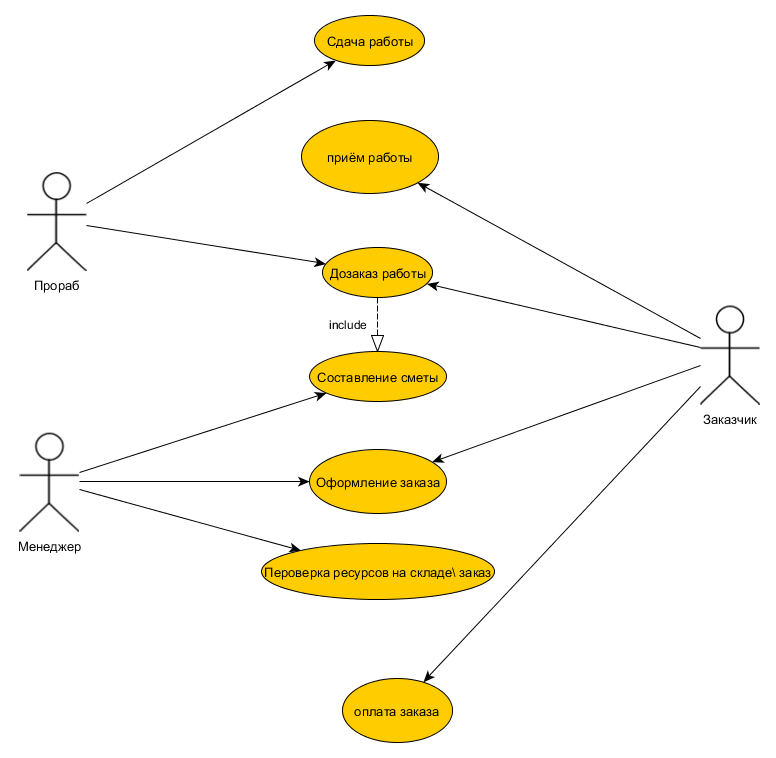
\includegraphics[width=0.7\textwidth]{img/uml_use_case.png}
	\caption{диаграмма вариантов использования}
\end{figure}
\newpage
\subsection{Описание вариантов использования}
\begin{enumerate}
\item Менеджер
	\begin{itemize}
		\item \textbf{Создание заказа.}
Менеджер создаёт новый заказ со статусом "открытый" и формирует смету после чего заказ переводится в состояния "в разработке" .
		\item \textbf{Создание сметы.} Менеджер прописывает все требуемые ресурсы и услуги оказываемые прорабом,
назначает прорабов для выполнения работ и передаётся список работ передаётся каждому из прорабов. Если ресурсов на складе не хватает то менеджер производит дополнительный заказ ресурсов.
		\item \textbf{Закрытие сметы.} После подтверждения оплаты от клиента смета переводится в статус "закрыта".
		\item \textbf{Закрытие заказа.} После оплаты всех смет заказ переводится в статус закрыт.
	\end{itemize}
\item Клиент
	\begin{itemize}
	\item \textbf{Оплата сметы.} Клиент оплачивает смету вводя часть либо полную стоимость сметы, если клиент оплачивает смету полностью то она пишется как оплаченная, если частично то стоимость сметы уменьшается на величину оплаты.
	\item \textbf{Принятие работы выполненной прорабом.} Завершение сметы, клиент принимает работу прораба и если все работы выполнены смета переходит в состояние "завершена" смету .
	\end{itemize}
\item Прораб
	\begin{itemize}
	\item \textbf{Завершение работы.} Прораб помечает работу выполненной,данную операцию можно выполнить если статус заказа которому принадлежит работа является "в разработке".
	\end{itemize}
\end{enumerate}
\newpage
\begin{figure}[!ht]
	\centering
	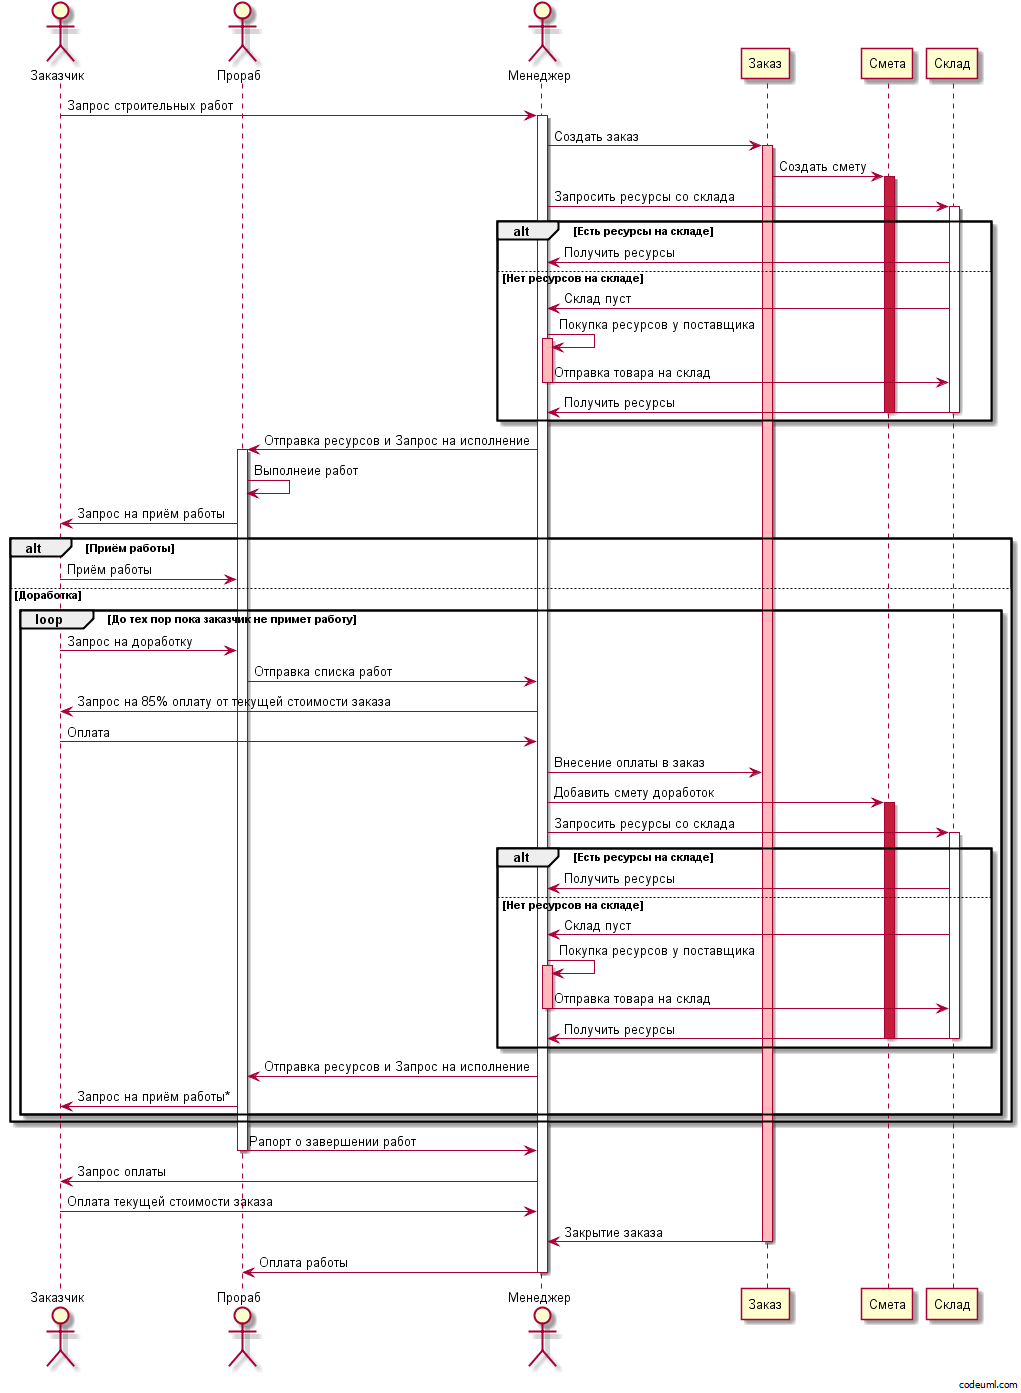
\includegraphics[width=0.9\textwidth]{img/getimage.png}
	\caption{диаграмма вариантов использования}
\end{figure}
\newpage
\subsection{Модель предметной области}
\begin{figure}[!ht]
	\centering
	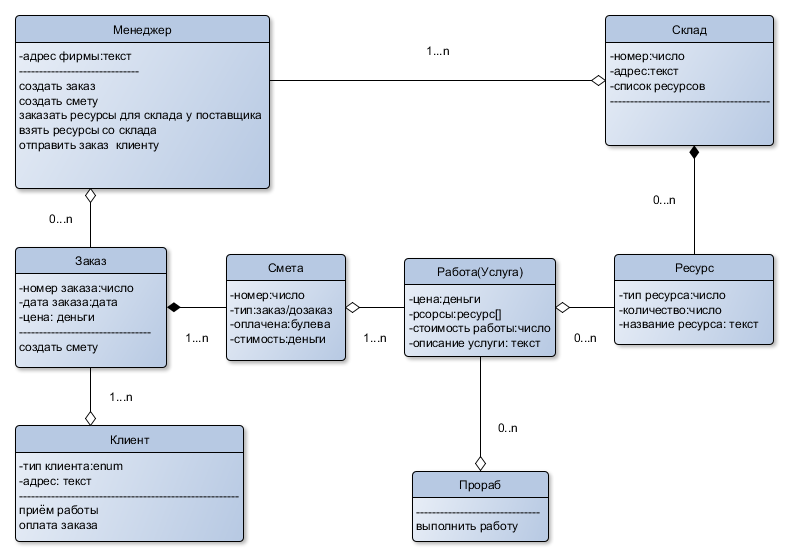
\includegraphics[width=0.9\textwidth]{img/uml_class_diagram.png}
	\caption{uml диаграмма классов}
\end{figure}
\subsection{Диаграмма последовательности}
\begin{figure}[!ht]
	\centering
	\includegraphics[width=1\textwidth]{img/diag1.png}
	\caption{Диаграмма последовательности менеджера}
\end{figure}
\newpage
\begin{figure}[!ht]
	\centering
	\includegraphics[width=0.6\textwidth]{img/diag2.png}
	\caption{Диаграмма последовательности заказчика}
\end{figure}
\begin{figure}[!ht]
	\centering
	\includegraphics[width=0.6\textwidth]{img/diag3.png}
	\caption{Диаграмма последовательности прораба}
\end{figure}
\newpage
\section{Архитектура}
\subsection{Общая архитектура проекта}
\begin{figure}[!ht]
	\centering
	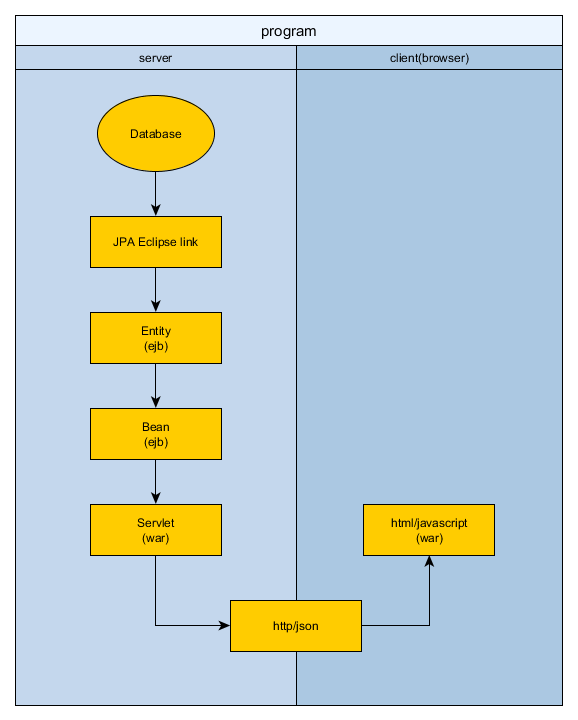
\includegraphics[width=0.6\textwidth]{img/architecture.png}
	\caption{архитектура клиент-серверного приложения}
\end{figure}

В качестве типового решения бизнес-логики была выбрана модель предметной области(Domain Model). Классы бизнес логики соответствуют uml диаграмме (рис.2) c дополнительными расширениями.
Бизнес логика расположена в разделе Entity (рис.4), взаимодействие с базой данных(слой хранения) осуществлено через ORM - EclipseLink по средством аннотаций. Авторизация пользователей осуществляется через механизм JAAS (Java Authentification and Authorization Service) логика управления в разделе Servlet.
\newpage
\subsection{Сущности, данные}
\textbf{Сущности - объекты с которыми работают роли:}

\begin{itemize}
\item Order - Заказ
\item Estimate - Смета в заказе
\item Storage - Склад содержащий список с ресурсами.
\item Work - Работы содержащие список ресурсов
\item Resource - Ресурсы.
\end{itemize}

\begin{itemize}
\item Manager - Роль менеджера.
\item Client - Роль заказчика
\item Master - Роль прораба
\end{itemize}

\textbf{Представление таблиц в базе данных.}

Таблицы:
\begin{itemize}
\item StorageList - информация о складе ресурсах на складе.
\item Storage - информация о складе.
\item Resource - информация о ресурсе его количестве и цене.
\item ResourceInformation - информация о ресурсах название и код ресурса.
\item Work - информация о работе и ответственном за неё прорабе.
\item WorkInformation - информация о стоимости работы(без стоимости ресурсов) и её описание
\item WorksAndResource - информация о ресурсах и их количестве нужном для работы.
\item Estimate - информация о списке смет для заказов.
\item EstimateWorks - информация о списке работ для смет.
\item Order - информация о заказе.
\item Manager - информация о менеджерах.
\item Master - информация о прорабах.
\item Client - информация о заказчиках.
\item Users - информация о пользователях системы (содержит пароль и логин пользователя).
\item Groupusers - сопоставляет пользователя и его роль в системе.
\end{itemize}

\begin{figure}[!ht]
	\centering
	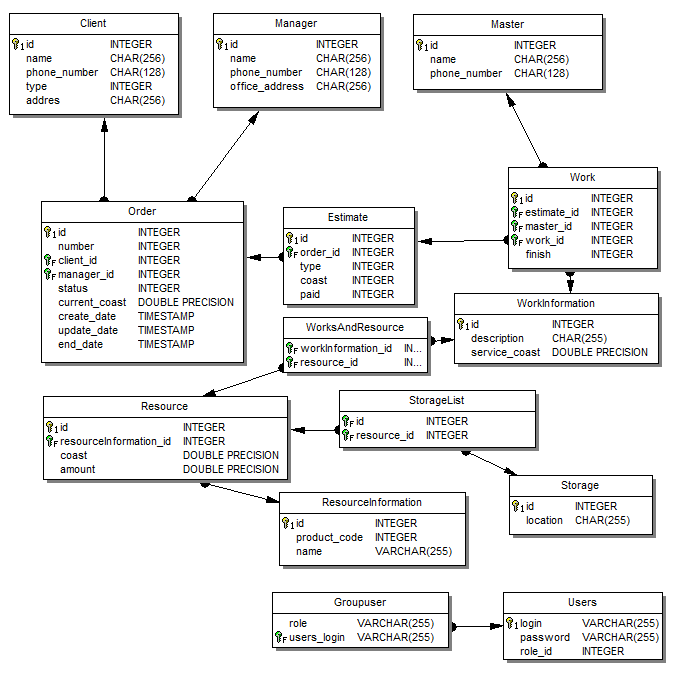
\includegraphics[width=0.7\textwidth]{img/database.png}
	\caption{таблицы в базе данных}
\end{figure}

\subsection{Пакеты и UMl диаграммы классов}
Проект состоит из пакетов:
\begin{itemize}
\item Entity сущности бизнес логики, а так же для работы с ORM через JPA по средством аннотаций.
\item Bean составляющих бизнес логику помещённую в EJB-Container.
\item API для взаимодействия с web клиентом через REST API(get,put,delete http запросы)
\item Sever для указания на какую страницу сайта перейти для конкретной роли.
\item Web графическая часть клиента html, css, javascript.
\end{itemize}
В диаграммах не указана графическая составляющая проекта html страницы с javascript кодом и фреймворком Angular JS, скриншоты из браузера для каждой роли можно увидеть в п.6
Диаграммы были созданы при помощи плагина NetBeanse easyUML.
\newpage
\subsubsection{Entity}
Ниже приведена диаграмма из пакета entity отражающего сущности указанные выше в п.3.2
взаимодействие между сущностями совпадает с зависимостями первичных и вторичных ключей между таблицами в базе данных, интерфейс converter нужен для преобразования данных в json формат и обратно методами toJSON - для получения данных в формате json и fromJSON - для преобразования из json в сущность. Класс Users не связан с остальными сущностями т.к. является вспомогательным для определения какой конкретной записи (в Client,Menager,Master) соответствует пользователь авторизировавшийся на сайте.
\begin{figure}[!ht]
	\centering
	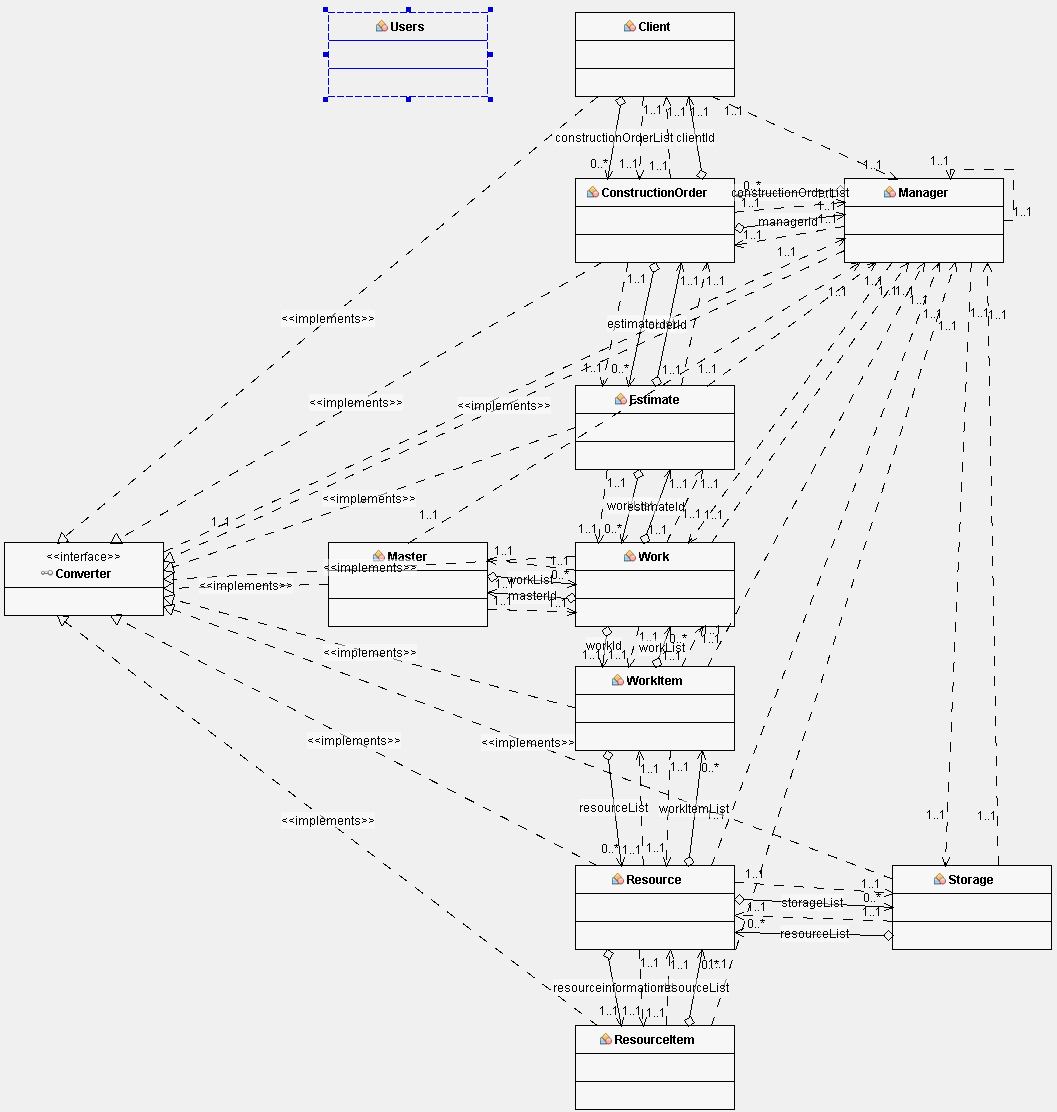
\includegraphics[width=1\textwidth]{img/entity.png}
	\caption{диаграмма классов из пакета entity}
\end{figure}
\subsubsection{Bean}
Было решено использовать 3 @Stateless bean-а соответствующих ролям в проекте, каждый класс отвечает за свою роль, общие методы для всех ролей были выведены в абстрактный класс AbstractRole, а так же обобщенный вывод для всех интерфейсов ролей был указан в BeanRemote методы которые не могут быть реализованы(некоторые методы реализация которых противоречит или нарушает целостность и безопасность логики приложения. Например роль клиента не имеет права вносить правки в стоимость сметы или заказа это может только менеджер или указывать завершение работы за что ответственен прораб) вызывают UnsupportedOperationException с соответствующим пояснением. Некоторые из json объектов не являются сущностями, а командами для выполнения бизнес логики обрабатываются в реализации метода.
\begin{figure}[!ht]
	\centering
	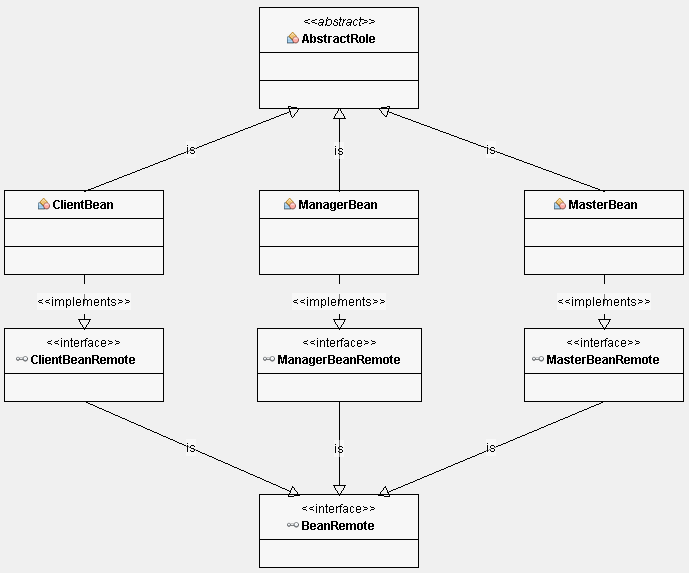
\includegraphics[width=0.7\textwidth]{img/bean.png}
	\caption{диаграмма классов из пакета bean}
\end{figure}
\newpage
\subsubsection{REST API}
В пакете api реализация REST API для управления из web клиента по средством get, put и delete http запросов передающих json данные. Для авторизации клиента и подачи ему страницы с соответствующей ролью используется класс AuthenticationServlet из пакета server
\begin{figure}[!ht]
	\centering
	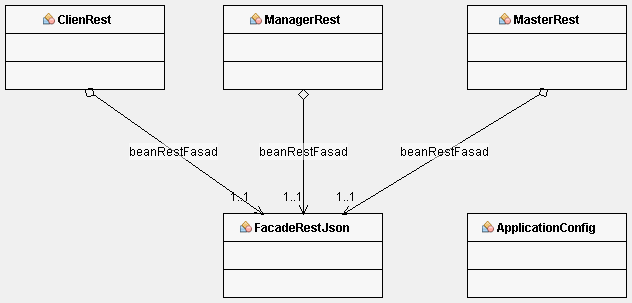
\includegraphics[width=0.7\textwidth]{img/api.png}
	\caption{диаграмма классов из пакета api}
\end{figure}


\textbf{REST API}\\\\
\textbf{\textbraceleft path\textbraceright} - обозначает url приложения, путь до приложения.\\\\
\textbf{для get запросов:}\\
\begin{itemize}
\item \textbf{\textbraceleft path\textbraceright /api/\textbraceleft role\textbraceright} - для получения общей информации связанной с данным пользователем, role - соответствует роли пользователя, может принимать значения manager,client,master. пример для manager см. рис. 11
\item \textbf{\textbraceleft path\textbraceright /api/\textbraceleft role\textbraceright /profile} - сведения о данном пользователе, ф.и.о. телефон и т.п. см. рис. 10
\item \textbf{\textbraceleft path\textbraceright /api/\textbraceleft role\textbraceright /array/\textbraceleft name\textbraceright} - для поучения массива объектов принадлежащих сущности, где name, это название массива сущности которые могут быть доступны для роли.
Для роли master доступен только массив works - список работ для данного прораба, для роли client доступен только массив orders - список заказов данного заказчика. Для менеджера доступны все массивы.
\item \textbf{\textbraceleft path\textbraceright /api/\textbraceleft role\textbraceright /array\textbraceleft name\textbraceright /\textbraceleft id\textbraceright} - для поучения объекта из массива принадлежащего сущности по id в базе данных.
\end{itemize}
\textbf{\\для put:}\\
\begin{itemize}
\item \textbf{\textbraceleft path\textbraceright /api/\textbraceleft role\textbraceright /array\textbraceleft name\textbraceright} - для создания новой записи, доступно только для роли manager.
\item \textbf{\textbraceleft path\textbraceright /api/\textbraceleft role\textbraceright /array\textbraceleft name\textbraceright /\textbraceleft id\textbraceright /update} - обновление существующей записи массива. Для каждой роли доступны определённые массивы: для роли client только массив orders, для master массив works, для manager - любой из массивов данных.
\item \textbf{\textbraceleft path\textbraceright /api/\textbraceleft role\textbraceright /profile} - обновление для собственных данных роли.
\end{itemize}
\textbf{\\для delete:}\\
Доступны только для роли менеджера:
\textbf{\textbraceleft path\textbraceright /api/\textbraceleft role\textbraceright /array/\textbraceleft name\textbraceright /\textbraceleft id\textbraceright}
может удалять элементы из любого массива сущностей.\\\\


\textbf{JSON} - поля объектов соответствуют записям базы данных (исключение это команды для обновления записей выполненные от роли клиента и прораба) массивы объектов это название сущности в множественном числе например для получения записи о клиентах используя роль менеджера при запросе\\
\textbf{\textbraceleft path\textbraceright /api/manager/array/clients} мы получим записи в масиве clients см. рис. 9
\begin{figure}[!ht]
	\centering
	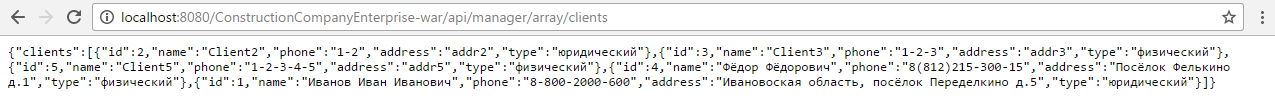
\includegraphics[width=0.9\textwidth]{img/api_json_clients.png}
	\caption{json массив клиентов}
\end{figure}
\begin{figure}[!ht]
	\centering
	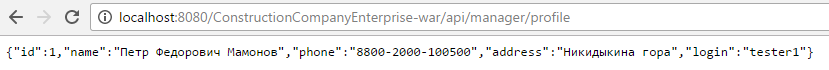
\includegraphics[width=0.9\textwidth]{img/api_profile.png}
	\caption{данные профиля пользователя}
\end{figure}
\begin{figure}[!ht]
	\centering
	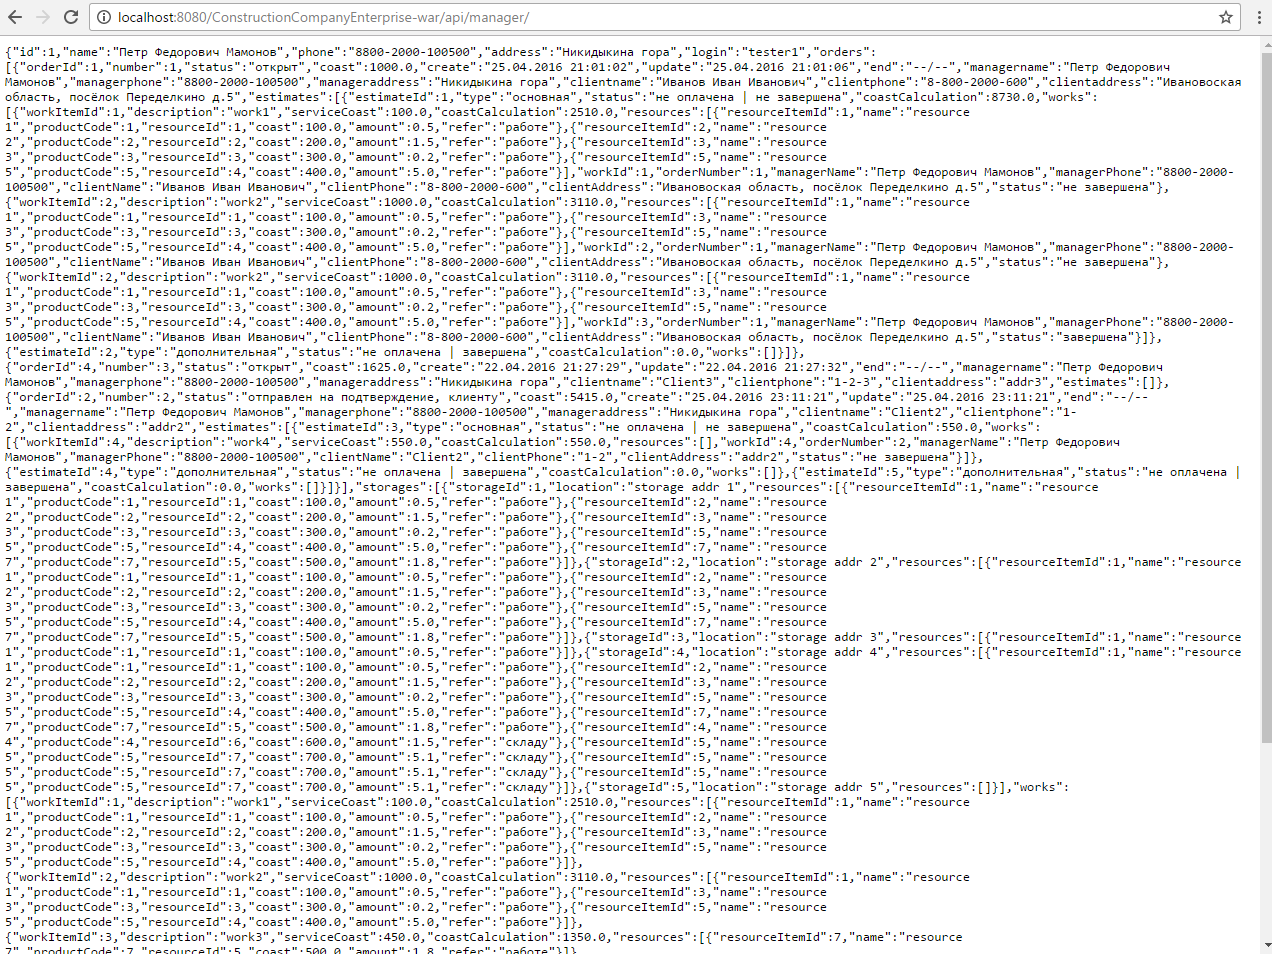
\includegraphics[width=0.9\textwidth]{img/api_manager_json.png}
	\caption{данные менеджера}
\end{figure}
\newpage
\section{Авторизация}
Авторизация осуществляется с помощью JAAS \\
(Java Authentification and Authorization Service). Во время авторизации пользователь посылает свои креденциалы (credentials, в простом случае это могут быть логин: пароль или пользовательский сертификат). На сервере с процессом контроля связаны две сущности, а именно Realm и Login Module. Login Module осуществляет проверку связи пользователя с каким-то набором групп пользователей (не путать с ролями). Кроме того, авторизация может быть пройдена успешно, однако, пользователь может быть не связан ни с одной из групп.

Веб-приложение может определять соотношение между группами и ролями. Приложение задаёт это соответствие с помощью web.xml.

Login Module и Realm не являются частью веб-приложения, а являются разделяемыми ресурсами сервера приложений, так что они должны быть в classpath сервера и должны быть соответствующим образом зарегистрированы в сервере (в login.conf и domain.xml). Приложение выбирает realm по имени через web.xml. 

Для GlassFish Server создать Realm через панель администратора указав источник для данных, это таблицы в базе данных с пользователями и ролями (есть и другие варианты, но в проекте был рассмотрен случай с базой данных как наиболее подходящий):
\begin{figure}[!ht]
	\centering
	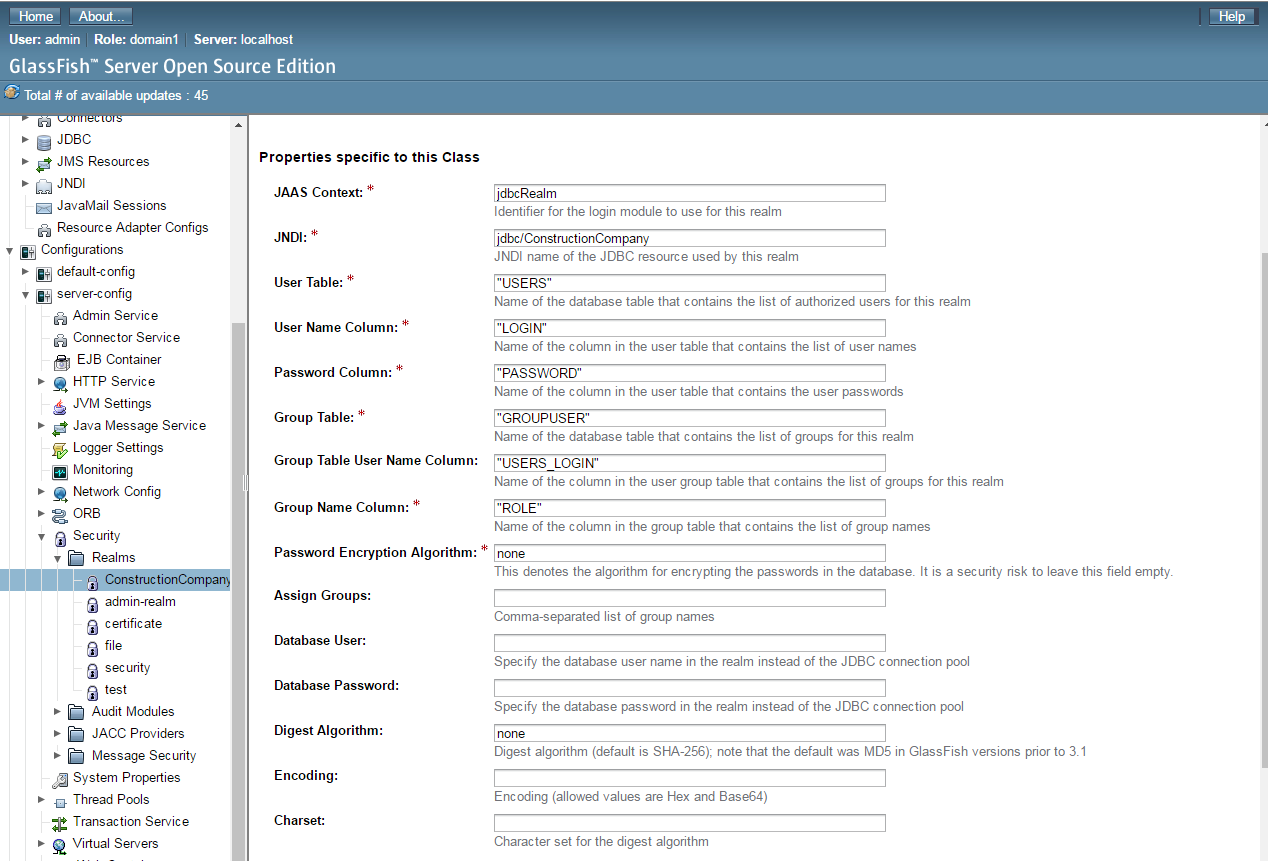
\includegraphics[width=0.8\textwidth]{img/security.png}
	\caption{раздел Realm для данного проекта}
\end{figure}
\begin{figure}[!ht]
	\centering
	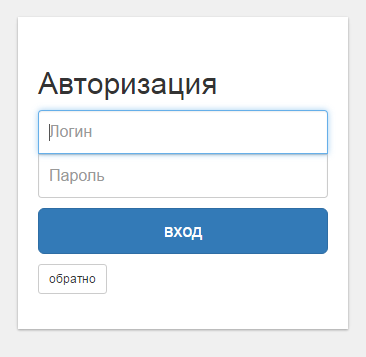
\includegraphics[width=0.3\textwidth]{img/auth.png}
	\caption{форма авторизации приложении}
\end{figure}
\newpage
\section{Тестирование}
Так как код бизнес логики был взят из прошлого проекта и все изменения не затронули поведение системы то на тестировании бизнес логики это не отражается.
\begin{figure}[!ht]
	\centering
	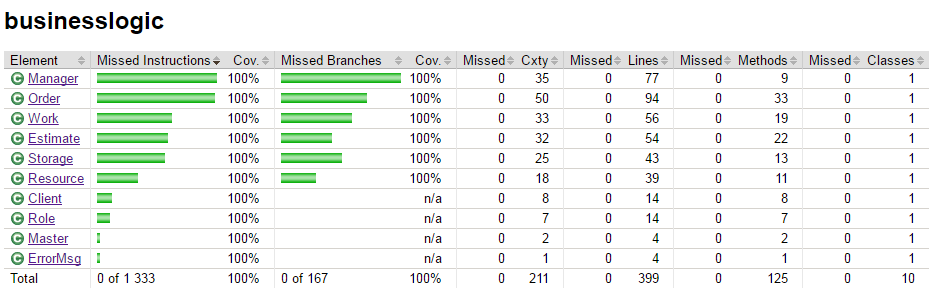
\includegraphics[width=0.8\textwidth]{img/busnesslogicJUintTest.png}
	\caption{тестовое покрытие бизнес-логики}
\end{figure}

\begin{center}
	\begin{longtable}{|p{0.3\linewidth}|p{0.3\linewidth}|p{0.3\linewidth}|}
		\hline
		\textbf{Вариант использования} & \textbf{Ожидаемый результат}&
		\textbf{Фактический результат}\\
		\hline
		Выбор сметы из списка заказов и нажатие кнопки Оплатить & После введения в диалоговом окне суммы для оплаты смета помечается как оплаченная & смета помечается как оплаченная на странице, а в случае полной оплаты заказа на странице менеджера заказ помечается как оплаченный и его статус переходит\\
		\hline
		Изменения в профиле и их сохранение  & Изменятся данные пользовательского профиля & Данные пользователя в базе данных изменятся на новые, так же это отобразит изменения в зависимых отображениях \\
		\hline
		Изменение статуса заказа по кнопке подтвердить & Заказ перейдёт из статуса <<отправлен на подтверждение, клиенту>> на <<на подтверждение оплаты, менеджеру>> & Статус заказа изменяется, на странице заказчика исчезает кнопка подтверждения а на странице менеджера появляется \\
		\hline
		\caption{Тестирование страницы заказчика}\\
	\end{longtable}
\end{center}


\begin{center}
	\begin{longtable}{|p{0.3\linewidth}|p{0.3\linewidth}|p{0.3\linewidth}|}
		\hline
		\textbf{Вариант использования} & \textbf{Ожидаемый результат}&
		\textbf{Фактический результат}\\
		\hline
		Выбор работы из списка и нажатие кнопки завершить & Работа помечается как завершённая & Работа помечается как завершенная, а так же проверяется статус выполнения сметы по количеству завершенных работ\\
		\hline
		Изменения в профиле и их сохранение  & Изменятся данные пользовательского профиля & Данные пользователя в базе данных изменятся на новые, так же это отобразит изменения в зависимых отображениях \\
		\hline
		\caption{Тестирование страницы прораба}\\
	\end{longtable}
\end{center}

\begin{center}
	\begin{longtable}{|p{0.3\linewidth}|p{0.3\linewidth}|p{0.3\linewidth}|}
		\hline
		\textbf{Вариант использования} & \textbf{Ожидаемый результат}&
		\textbf{Фактический результат}\\
		\hline
		Изменения состояния, добавления и удаления различных сущностей (ресурсы, работа, смета, заказ, заказчик, прораб, склад)  & После введения в диалоговом окне и проверки на не противоречивость данные сохраняются & Сущности изменяются в соответствии с заданными, в пределах ограничений области допустимых значений для данных\\
		\hline
		Изменения в профиле и их сохранение  & Изменятся данные пользовательского профиля & Данные пользователя в базе данных изменятся на новые, так же это отобразит изменения в зависимых отображениях \\
		\hline
		Изменение статуса заказа по кнопке закрыть & Заказ перейдёт из статуса <<на подтверждение оплаты, менеджеру>> на <<закрыт>> & Статус заказа изменяется, на странице менеджера исчезает кнопка подтверждения, а на странице заказчика статус заказа изменяется на закрыт \\
		\hline
		\caption{Тестирование страницы менеджера}\\
	\end{longtable}
\end{center}
\newpage
\section{Графика}
Скиншоты html страницы в браузере для каждой роли:
\begin{figure}[!ht]
	\centering
	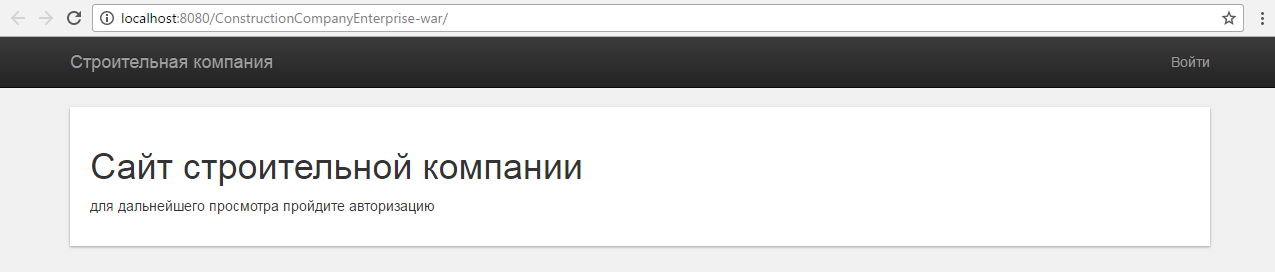
\includegraphics[width=0.9\textwidth]{img/main.png}
	\caption{приветственная страница}
\end{figure}
\begin{figure}[!ht]
	\centering
	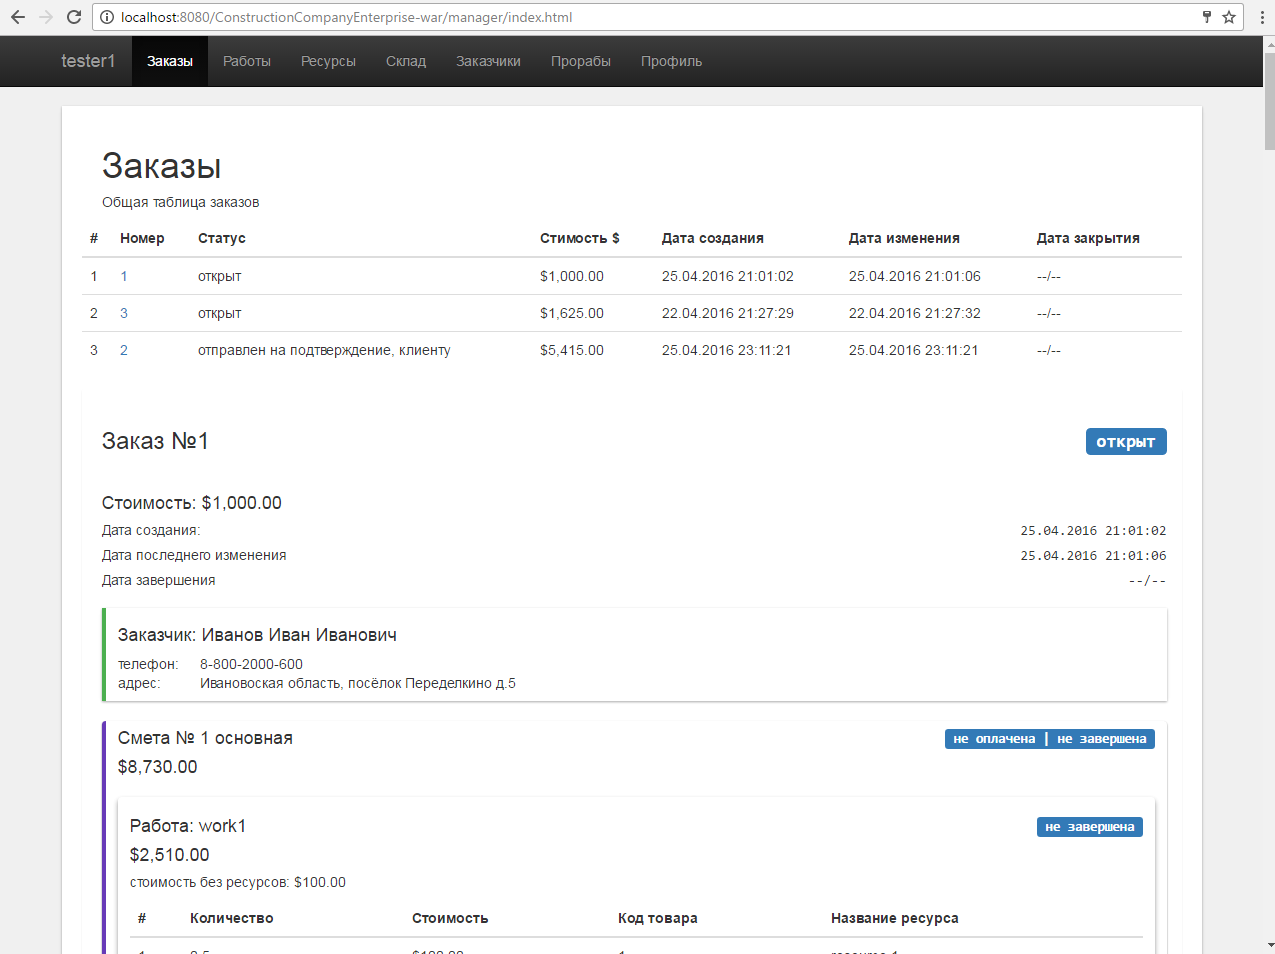
\includegraphics[width=0.9\textwidth]{img/manager.png}
	\caption{роль менеджера}
\end{figure}
\newpage
\begin{figure}[!ht]
	\centering
	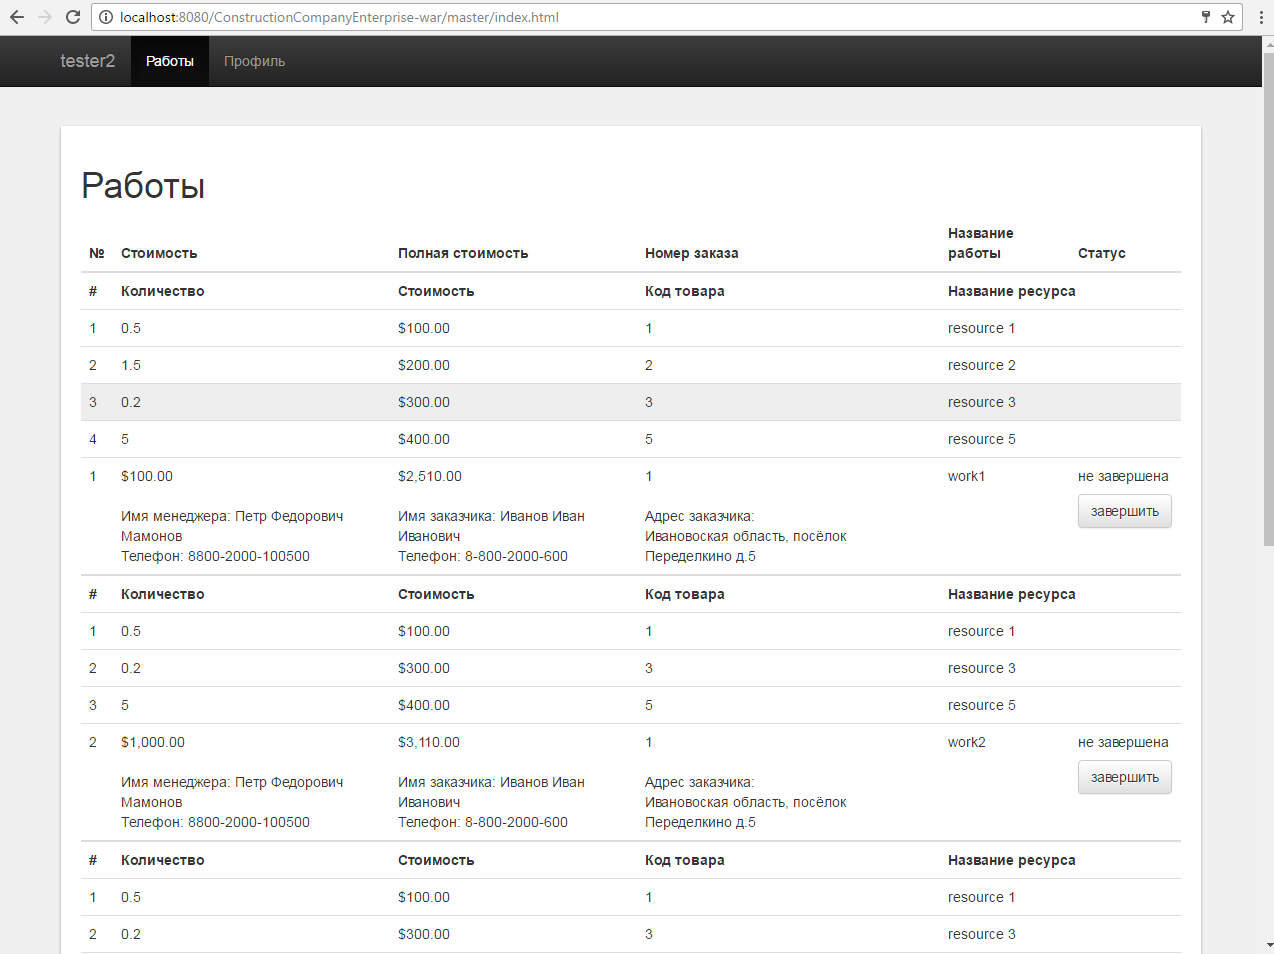
\includegraphics[width=0.8\textwidth]{img/master.png}
	\caption{роль прораба}
\end{figure}
\begin{figure}[!ht]
	\centering
	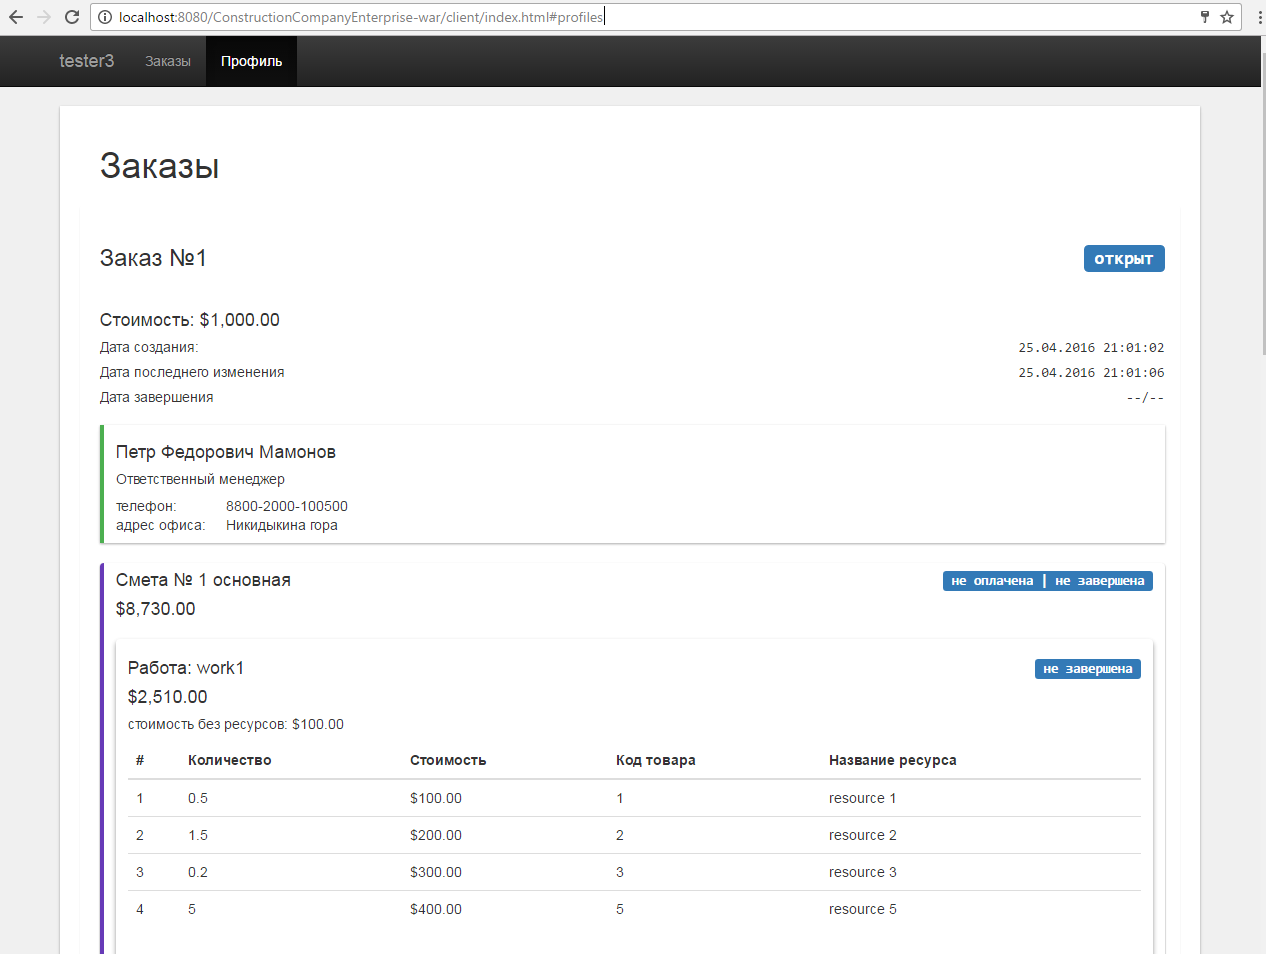
\includegraphics[width=0.8\textwidth]{img/client.png}
	\caption{роль заказчика}
\end{figure}
\begin{figure}[!ht]
	\centering
	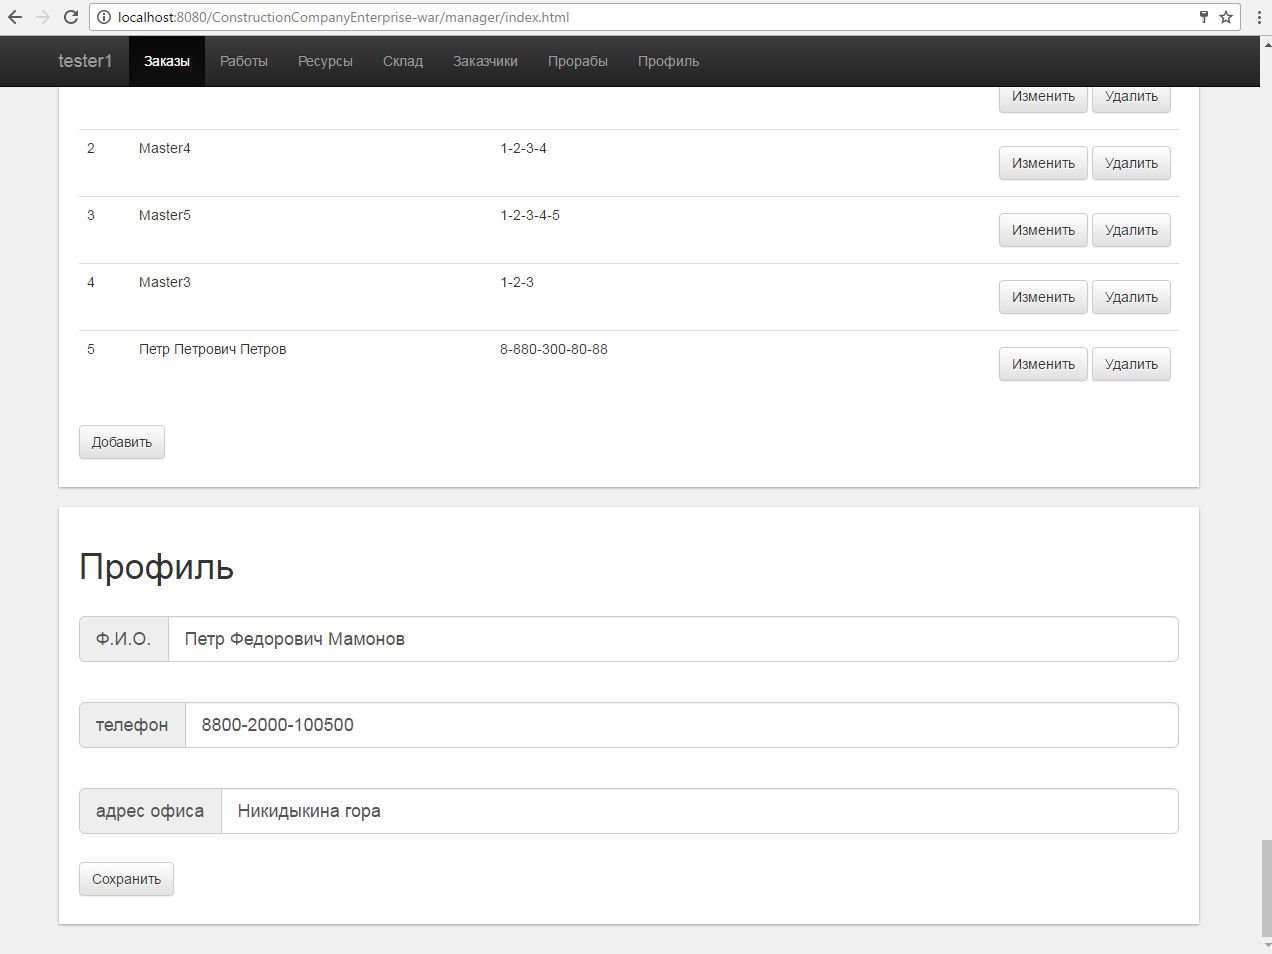
\includegraphics[width=0.8\textwidth]{img/profile.png}
	\caption{профиль менеджера}
\end{figure}
\newpage
\section{Выводы}
В качестве сервера приложений использовался GlassFish Server 4.1, в качестве ORM - EclipseLink
Для хранения данных использовалась СУБД PostgreSQL 9.6
Для web клиента использованы сторонние библиотеки :
\begin{itemize}
\item Angular JS для работы http запросов и отображения JSON данных полученных от сервера,чтобы сократить трафик обмена информацией между клиентом и сервером.
\item Для визуального стилистического оформления html страниц была использована библиотека Bootstrap 3.
\item Для работы фреймворка и библиотеки понадобилась подключить jQuery.
\end{itemize}
Данная работа моделирует пример проектирование архитектуры распределённой информационной системы для бизнес процессов на примере строительной организации. Были изучены технологии EJB (Enterprise Java Beans) и JPA (Java Persistence API).
